\documentclass[conference]{IEEEtran}  % Comment this line out
                                                          % if you need 
\usepackage{graphicx}
\usepackage{algorithm}% http://ctan.org/pkg/algorithm
\usepackage{algpseudocode}% http://ctan.org/pkg/algorithmicx
\usepackage{textcomp}
\usepackage{amssymb}
\usepackage{authblk}
\usepackage{caption}
\usepackage{subcaption}
\usepackage{subfig}
\usepackage{float}
\usepackage{array}
\usepackage{amsmath}
\usepackage{csquotes}

\makeatletter
\newcommand*{\rom}[1]{\expandafter\@slowromancap\romannumeral #1@}
\makeatother

\title{\LARGE \bf
Shapelets and Parallel Coordinates Based Automated Query Generation for Complex Event Processing
}

\author{R.N. Navagamuwa}
\author{K.J.P.G. Perera}
\author{M.R.M.J. Sally}
\author{L.A.V.N. Prashan}
\author{H.M.N. Dilum Bandara}
\affil[]{Department of Computer Science and Engineering\protect\\ University Of Moratuwa\protect\\ Katubedda, Sri Lanka \authorcr Email: {\tt (randika.12, pravinda.12, jaward.12, prashan.12, dilumb)@cse.mrt.ac.lk} \vspace{-2ex}} 

\begin{document}
\graphicspath{ {images/} }


\maketitle
\thispagestyle{empty}
\pagestyle{empty}


%%%%%%%%%%%%%%%%%%%%%%%%%%%%%%%%%%%%%%%%%%%%%%%%%%%%%%%%%%%%%%%%%%%%%%%%%%%%%%%%
\begin{abstract}

Automating the query generation for Complex Event Processing (CEP) has marked its own importance in allowing users to obtain useful insights from data. Existing techniques are both computationally expensive and require extensive domain-specific human interaction. In addressing these issues, we propose a technique that combines both parallel coordinates and shapelets. First each instance of the multivariate data is represented as a line on a set of parallel coordinates. Then a shapelet-learner algorithm is applied to those lines to extract the relevant shapelets. Afterwards, the identified shapelets are ranked based on their information gain. Next, the shapelets with similar information gain are divided into groups by a shapelet-merger algorithm. The best group for each event is then identified based on the event distribution of the dataset. Then the best group is used to generate the query to detect the complex events. The proposed technique can be applied to both multivariate and multivariate time-series data, and it is computationally and memory efficient. It enables users to focus only on the shapelets with relevant information gains. We demonstrate the utility of the proposed technique using a set of real-world datasets.  

\end{abstract}

\begin{IEEEkeywords} 
Complex Event Processing, Multivariate Time Series, Parallel Coordinates, Shapelets
\end{IEEEkeywords}

%%%%%%%%%%%%%%%%%%%%%%%%%%%%%%%%%%%%%%%%%%%%%%%%%%%%%%%%%%%%%%%%%%%%%%%%%%%%%%%%
\section{Introduction}

Automating query generation in large, multivariate datasets are useful in many applicationu domains. For example, Complex Event Processing (CEP) \cite{IEEEexample:CEP} combines data from multiple, streaming sources to identify meaningful events or patterns in real time. While the detection of relevant events and patterns may give insight about opportunities and threats related to the data being monitored (e.g., set of sensor readings and credit card transactions), significant domain knowledge is required to write effective CEP queries. Manual analysis of data streams is not only tedious and error prone, but also important events are likely to be missed due to the limited domain knowledge of the query writer. A promising alternative is to automate the CEP query generation by automatically extracting/mining interesting patterns from the past data \cite{IEEEexample:autoCEP,IEEEexample:TowardsAutomated,IEEEexample:LearningFromThePast}.

Time-series pattern mining and classification techniques are extensively studied in the literature. Dynamic Time Warping (DTW) \cite{IEEEexample:DTW} is one such technique used to measure the similarity between two time series based on a distance measure. However, the computational complexity of DTW grows exponentially with large and multiple time series limiting its usages. Moreover, the accuracy of the results depends on the chosen sliding window, which is nontrivial to estimate \cite{IEEEexample:autoCEP}. A shapelet \cite{IEEEexample:TimeSeriesShapelets} is a time series subsequence that is identified as being representative of class membership; hence, useful in time-series classification. AutoCEP \cite{IEEEexample:autoCEP} proposed a shapelet-based technique to automate the CEP query generation for univariate time series. This itself is a major limitation as the practical presence of univariate time series is limited in CEP. Moreover, AutoCEP generates queries for each and every instance of the detected event, requiring the CEP engine to concurrently process multiple queries. This unnecessarily increases the computational and memory requirements of the CEP engine and consequently degrades its performance. One trivial optimization is to use the assistance of a domain-expert to aggregate the queries and attempt to write one or few queries. Ultra-fast shapelets \cite{IEEEexample:UltraFast} are proposed for multivariate time-series classification. Ultra-fast shapelets calculates a vectorized representation of respective attributes of the dataset. Then a random forest is trained to identify the shapelets with respect to the total dataset. The leaves of the random forest are considered to be the symbols. The number of occurrences of a symbol in the raw data is counted and these symbol histograms are used for the final classification using random forests. While this technique is effective in classification, it cannot be used to generate CEP queries, as the generated random forest does not support backtracking and obtaining any relevant information as to what data lead to the classification of the event \cite{IEEEexample:UltraFast}. Rare itemset pattern mining (AprioriRare) \cite{IEEEexample:RareItemSet} is another technique. This technique cannot be used to detect events that occur within a short period of time. Moreover, most related work focus only on domain-specific datasets limiting the usability across diverse datasets and applications \cite{IEEEexample:UserOriented,IEEEexample:WebBased}.

We propose a technique that represents the given multivariate dataset as a set of parallel coordinates, and then extract shapelets out of those coordinates to auto generate CEP queries. Even a time series can be mapped to a set of parallel coordinates, by representing each time instance as a separate line. Extracted shapelets are sorted according to the information gains and then divided into a several groups. Out of the all groups, best group for each event is identified. Then the most important shapelets in the identified groups are used to generate one CEP query per group. This enables one to generate CEP queries for commonalities, anomalies, as well as time-series breakpoints in a given multivariate time-series dataset without having any domain knowledge. Users can focus on groups with high or low information gain depending on the application. Moreover, shapelets identify most relevant attributes in a dataset for a particular event, enabling us to write more efficient CEP queries and only one query per event (unless the same event is triggered by unrelated attribute combinations). Using a set of real-world datasets, we demonstrate that the proposed technique can be applied effectively to auto generate CEP queries for common and abnormal events while identifying the relevant features and event occurrence timeframe. Moreover, the proposed technique has a relatively low computational and memory requirements compared to prior work.

Rest of the paper is organized as follows. Section II introduces shapelets, parallel coordinates, and problem formulation. Section III presents the proposed technique and Section IV explains implementation details. Performance analysis is presented in Section V. Concluding remarks and future work are discussed in Section VI.

\section{Preliminaries}
We first define relevant terms and then define shapelets and parallel coordinates as applicable to the domain of CEP query generation. The research problem is then formulated.
\subsection{Definitions}
\textbf{\textit{Time-Series}} --- A time-series $T = t\textsubscript{1},..., t_m$ is an ordered set of \textit{m} real-valued variables.
\smallskip\\
\textbf{\textit{Multivariate Time-Series}} --- A multivariate time-series $T = t\textsubscript{1}, . . . , t_m$ is a sequence of \textit{m} vectors, where $t_i = (t_{i,1}, . . . , t_{i,s})$ $\epsilon$ $\mathbb{R}\textsuperscript{\(s\)}$ with \textit{s} attributes/variables.
\smallskip\\
\textbf{\textit{Sub-sequence ($S^t_p$)}} --- Given a time-series $T$, a subsequence $S^t_p$ of $T$ is a sampling of length $l$ \(\leq\) $m$ of contiguous positions from $T$ starting at time $p$, i.e., $S^t_p = t_p, t_{p+1}...,t_{p+l-1}$, for 1 \(\leq p \leq m - l + 1\).
\smallskip\\
\textbf{\textit{Set of All Sub-sequences ($ST_l$)}} --- Set of all possible sub-sequences $S^t_p$ that can be extracted by sliding a window of length $l$ across $T$ is $ST_l$ = \{all $S^t_p$ of $T$,  for 1 \(\leq p \leq m - l + 1\)\}.
\smallskip\\
\textbf{\textit{Sub-sequence Distance}} --- Given $T$ and $S^t_p$ \(SubsequenceDist(T,S^t_p)\) is the minimum distance between $p$ contiguous positions obtained by sliding $S^t_p$ across $T$. We use Euclidean distance as the distance function.
\smallskip\\
\textbf{\textit{Entropy}} --- A time series dataset \textbf{D} consists of two classes, $A$ and $B$. Given that the proportion of objects in class $A$ is $p(A)$ and the proportion of objects in class $B$ is $p(B)$, the entropy of \textbf{D} is
\begin{equation}
 I(\textbf{D}) = -p(A)log(p(A))  - p(B)log(p(B))
 \label{eq:id}
\end{equation}
\smallskip\\
\textbf{\textit{Information Gain (Gain)}} --- Given a certain split strategy $sp$ which divides \textbf{D} into two subsets \textbf{D\textsubscript{1}} and \textbf{D\textsubscript{2}},the entropy before and after splitting is $I(\textbf{D})$ and $\hat{I}(\textbf{D})$. For a split $sp$ of the dataset the information gain is:
\begin{equation}
\begin{split}
Gain(\textit{sp}) = I(\textbf{D}) - \hat{I}(\textbf{D})\\
Gain(\textit{sp}) = I(\textbf{D}) - (f(\textbf{D\textsubscript{1}})(I\textbf{D\textsubscript{1}})+f(\textbf{D\textsubscript{2}})I(\textbf{D\textsubscript{2}}))
\end{split}
\label{eq:gain}
\end{equation}
Here $f(\textbf{D})$ is defined as the fraction of objects in \textbf{D}. 
\smallskip\\
\textbf{\textit{Optimal Split Point (OSP)}} --- Consider a time-series dataset \textbf{D} with two classes $A$ and $B$. For a given $S^t_p$, we choose some distance threshold $d_{th}$ and split \textbf{D} into \textbf{D}\textsubscript{1} and \textbf{D}\textsubscript{2}, s.t. for every time series object $T_{1,i}$ in \textbf{D}\textsubscript{1}, \(SubsequenceDist(T_{1,i}, S^t_p) \leq d\textsubscript{th}\) and for every $T_{2,i}$ in \textbf{D}\textsubscript{2}, \(SubsequenceDist(T_{2,i}, S^t_p) \geq d\textsubscript{th}\). An Optimal Split Point (OSP) is a distance threshold that \( Gain(S^t_p,d\textsubscript{OSP(D,$S^t_p$}) \geq Gain(S^t_p,d'_{th}) \) for any other distance threshold $d'_{th}$.
\subsection{Shapelets}
\textit{Shapelets} can be defined as time-series sub-sequences as seen in Fig.~\ref{fig:shapelets}. 
%A dataset can be converted to two dimensional representation of time series \cite{IEEEexample:TimeSeriesShapelets}. This representation can be used for time-series classification based on the shapes of the data within the time series. For example, many subsequences can be identified on a time series , and those subsequences are called shapelets. 
Shapelets can be of varying lengths, and many sub-sequences can be extracted by sliding a window of given length $l$. In shapelet-based classification, the objective is to identify a shapelet that is in some sense maximally representative of a class.
%and all possible subsequences can be extracted using sliding window as illustrated in Fig. 2.
%\smallskip\\
%\begin{figure}
%\centering
%\begin{minipage}{9cm}
%\parbox{9cm}{
%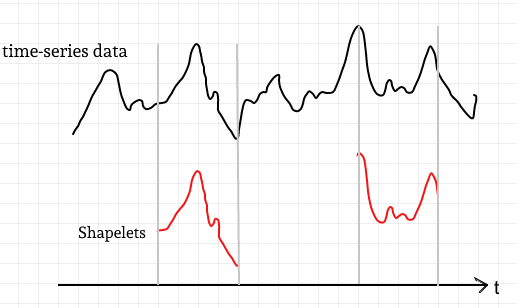
\includegraphics[width=9cm,height=3cm]{shapelet1.png}
%\caption{Time-series shapelets.}
%\label{fig:2figsA}}
%\qquad
%\parbox{9cm}{
%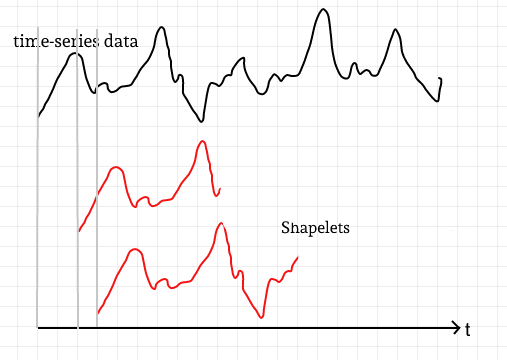
\includegraphics[width=9cm,height=4cm]{shapelet2.png}
%\caption{Shapelets with sliding window.}
%\label{fig:2figsB}}
%\end{minipage}
%\end{figure}

\begin{figure}
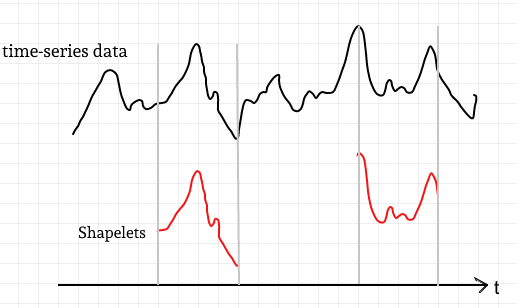
\includegraphics[width=9cm,height=3cm]{shapelet1.png}
\caption{Time-series shapelets.}
\label{fig:shapelets}
\end{figure}

\subsection{Parallel Coordinates}
Parallel coordinates are widely used to visualize multivariate data \cite{IEEEexample:ParallelCoordinates}. Fig.~\ref{fig:parallcor}. Fig.~\ref{fig:parallcor} illustrates the parallel coordinates representation of the room occupancy dataset obtained from the UCI Machine Learning repository \cite{IEEEexample:Ocupancy}. The complete dataset is visualized in grey colour and a selected set of data instances in black colour. Dataset with $n$ dimensions (i.e., attributes) is mapped to a set of points on $n$ parallel lines, where each line represents an instance of data. These points are then connected using a line. A separate line is drawn for each instance of data (i.e., each row). When scaling these coordinate systems, it is recommended to use normalized data to prevent bias to certain dimensions.
\begin{figure}
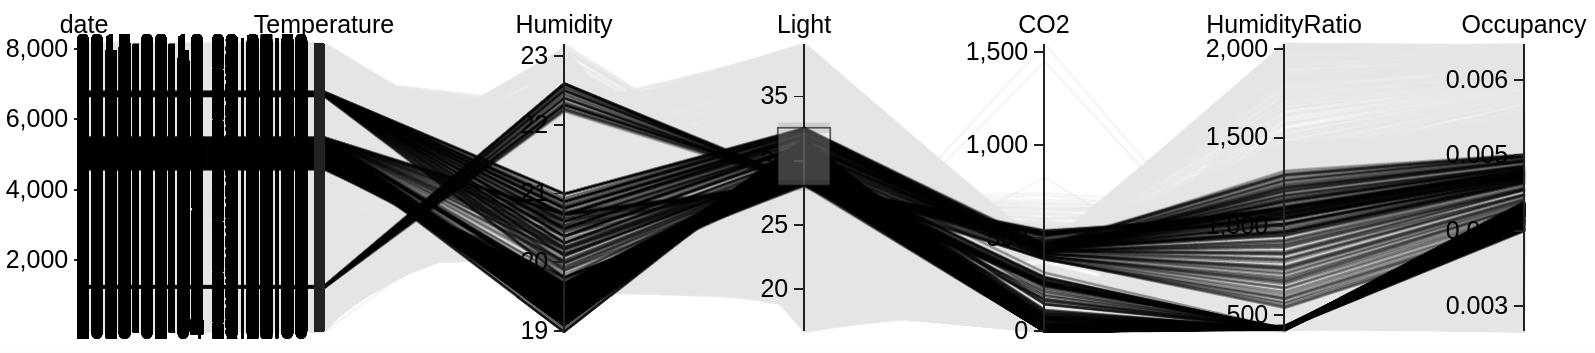
\includegraphics[width=9cm,height=4cm]{occupancy_d3.png}
\caption{Parallel coordinates representation of Occupancy Detection dataset \cite{IEEEexample:Ocupancy}.}
\label{fig:parallcor}
\end{figure}

\subsection{Problem Statement} 
In contrast to relational database systems that issue dynamic queries on stored and indexed data, CEP filters incoming streams of data through pre-written queries to detect events of interest. Hence, relevant queries need to be provided to the CEP engine a priori. We address the problem of needing domain knowledge to write a meaningful CEP queries through automation. Though a couple of related work attempt to automate CEP query generation, they support only univariate time series data \cite{IEEEexample:autoCEP}.

We propose a solution which can be used to generate CEP queries for multivariate time series without requiring expert domain knowledge. In proposing the solution we assume that each instance in the obtained dataset is annotated according to the respective event. Our goal is to construct a filter query per event, which contains the most relevant attributes, their range of values, and the event detection time frame, e.g., a sample CEP filter query may look like the following:

\begin{equation}
\begin{split}
\textbf{SELECT }\ \{*\} \\ \textbf{WHERE}\ \{attr_1\geq a\ and \ attr_2<b\} \\ \textbf{WITHIN}\ \{t_1\leq time\leq t_2\}
\label{eq:query}
\end{split}
\end{equation}

\begin{figure}
\includegraphics[width=0.5\textwidth]{High_level_architecture.png}
\caption{High-level architecture of the proposed solution.}
\label{fig:archi}
\end{figure}

\section{Proposed Technique}
To auto generate queries for Complex Event Processors, we propose the modularized architecture illustrated in Fig.~\ref{fig:archi}. The four main modules perform the following tasks:

\textbf{Data Processor} --- Converts the input dataset (e.g., time series data in .txt, .xml, or .csv format) into a generic format used by rest of the modules. We assume that each instance in the given dataset corresponds to an occurrence of a specific event, i.e., each data instance is classified/labeled with the corresponding event. The module then counts the number of events of each type, and their proportions with respect to the total number of events in the entire dataset.

\textbf{Shapelet Generator}	--- This is the core module of the system which uses pattern mining. This module identifies the most appropriate shapelets to represent each event. First, the multivariate time series dataset is mapped to a set of parallel coordinates. Fig.~\ref{fig:tsdata} illustrates an exemplary representation of a multivariate time series with six attributes and six time instances converted to parallel coordinates. Then all the shapelets are extracted from the parallel coordinates while varying the length $l$ of the sliding window. Though the shape of the extracted shapelets depend on the order of the attributes, final outcome of the solution is independent of the order. Length of an identified shapelet is bounded by number of attributes $m$ in the time series (i.e., $1 \leq l \leq m$). Therefore, our technique produces a much lower number of shaplets compared to prior work, where $m$ can be as large as the length of the time series. Moreover, it is not required to apply heuristics or expert knowledge to determine the optimum minimum and maximum length of shapelets. Therefore, our \textit{Shapelet Learner Algorithm} is both computationally and memory efficient.

Once all shapelets are extracted, the next step is to identify a subset of the shapelets that are representative of patterns in the parallel coordinates. For this, we use information gain, which is an estimate of the extent that a selected shapelet is similar to a given line on parallel coordinates. For example, Fig.~\ref{fig:tsshapes} shows two shaplets, one with attributes 1 and 2 (shapelet $S_1$) and another with attributes 1, 2, and 3 (shapelet $S_2$). We slide both $S_1$ and $S_2$ across the line/row with $t$ = 0, and find the minimum distance between the shapelet and line. For example, $S_1$ has a relatively lower distance between the attributes 1-2 and 3-4, whereas $S_2$ has a relatively lower distance between attributes 1-3 and 4-6. This is estimated using the \textit{SubsequenceDist()} function defined in Sec. 2.1. The same process is applied to all other time instances and shapelets. This results in an array for shapelets and corresponding minimum distance for each time instance. We then find the Optimal Splitting Point (OSP) \cite{IEEEexample:TimeSeriesShapelets} for each array of minimum distances, to find the maximum information gain for each shapelet. The shapelets are then ranked based on the descending order of its information gain. We then use \textit{Shapelet Merger Algorithm} to group shapelets within the ranked list with respect to their information gain. Because the shapelets with similar information gains produce similar insights, groups created using \textit{Shapelet Merger Algorithm} allows us to cluster the similar informative shapelets together. Finally, \textit{Important Shapelet Extraction Algorithm} is used to identify the most suitable shapelets to represent each event type, which would result in an output similar to Fig.~\ref{fig:tswin}.

\textbf{Visual Representation} --- This module visualizes generated shapelets, optionally enabling users to select what shapelets to choose for query writing. While the system can auto generate queries without any user suggestions, this module facilitates and accepts user approval allowing the user to select the shapelets that user is interested in. As seen in Fig.~\ref{fig:tswin} user may also select subset of the attributes and their range of values that he/she expects to use in the generated queries. Such user intervention reduces false positives and improves performance of the CEP engine, as not every identified event may be of practical importance.

\begin{figure}
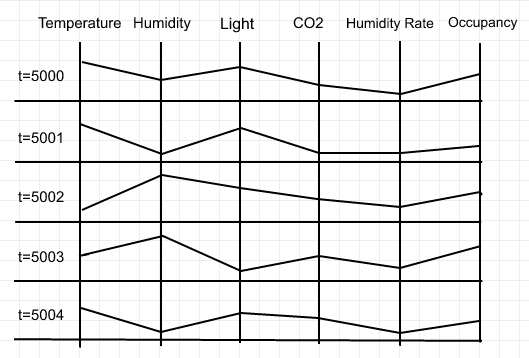
\includegraphics[width=9cm,height=5cm]{multivariateTime.png}
\caption{Multivariate time series mapped as parallel coordinates.}
\label{fig:tsdata}
\end{figure}

\begin{figure}
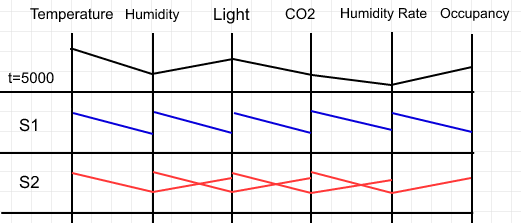
\includegraphics[width=0.5\textwidth]{movingWindow.png}
\caption{Shapelets slide accross the time series.}
\label{fig:tsshapes}
\end{figure}

\begin{figure}
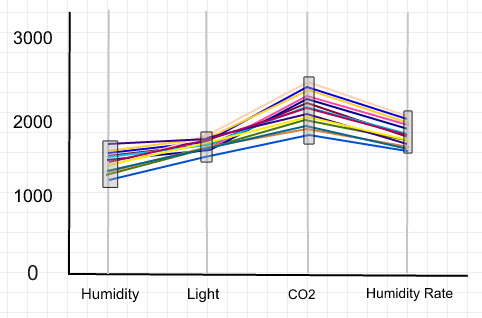
\includegraphics[width=0.5\textwidth]{demo.png}
\caption{Event representative shapelets.}
\label{fig:tswin}
\end{figure}

\textbf{Query Generator} --- Given the chosen shapelets this module auto generates CEP queries based on the input provided by the hint generator module and incorporating any user provided hints. Here we generate one query per each event with the relevant query parameters generated by the system, or set of attributes and ranges approved by the user. The module identifies the most relevant attributes and their value ranges to be used in constructing the query along with the optimal time periods within which each event occurs. Optimal time periods are generated analyzing the event distribution of the actual dataset and choosing the longest event detection time period with respect to each event occurrence. Using these data the module generates queries for each and every event of the given dataset and a generates a filter query similar to (3).

\section{Implementation}
%Few and recent efforts that touched about Shapelets are discussed in \cite{IEEEexample:TimeSeriesShapelets,IEEEexample:ExtractingShapelets,IEEEexample:autoCEP}. 
In this paper we introduce a new approach to define shapelets using parallel coordinates as an object with four attributes ${s = (g,i,a,c)}$. $g$ is the information gain, which measures the similarity between shapelet and time series. $i$ is the time series identifier, which is the row number of the line on parallel coordinates (see Fig.~\ref{fig:tsdata}). $a$ is the starting column/attribute number. We store the normalized values of the attributes which belong to the particular shapelet in $c$. In addition to the normalized values, we keep the original values as well( These original values will be used to generate the CEP query).

We first transform the multivariate time series dataset into parallel coordinates. For example, Fig.~\ref{fig:parallcor} depicts the parallel coordinates representation of Occupancy Detection dataset, which we use for the first performance study. Our method builds upon two main phases which are illustrated in Fig.~\ref{fig:hintgen}. Next, implementation of each phase is discussed in detail.
%We then extract all possible shapelets from the parallel coordinates representation. , and then identify important shapelets for further processing


\subsection{Phase one: Shapelet Learner}
The Shapelet Learner extracts all the shapelets from the obtained parallel coordinates. We set the default minimum length ($l{min}$) of a shapelet as two, while the maximum ($l{max}$) is set to the number of attributes $m$ (i.e., $2 \leq l \leq m$). However, a user may override these values. Afterwards, Algorithm 1 of the Shapelet Generator module extracts all possible shapelets while varying the shapelet length. First, the shapelet list is initialized to store the extracted shapelets (line 2). Then shapelets are extracted by going through each row $r$ in the Dataset \textbf{D}. The outer loop increments the length of a shapelet $l$ up to $l_{max}$, while the inner loop increments $start$ to scans through each $r$, and inner-most loop extract all attributes between $l_{min}$ to $l$ for a given staring point. Then we convert each shapelet’s content to standard normal using \textit{zNorm()} function to prevent any biases to specific attributes. Moreover, in line 19 we also store the raw values of shapelets, as they are later required while generating queries. 

We also calculate and save the information gain of each shapelets using \textit{infoGain()} function. \textit{infoGain()} function compares the shapelet with each and every row of the parallel coordinates. The minimum distance between the row and the shapelet is found by sliding the shapelet across the row, one attribute at a time (see Fig. \ref{fig:tsshapes}) and the minimum distance per each row is saved in an array, meaning there would be an array per each generated shapelet. Then by sequeuntially splitting the array we calculate the information gain. Finally for each shapelet we get the maximum information gain and the corresponding split point which would be the Optimum Splitting Point of the array. Each shapelet and its meta data are then added to the \textit{shapelets} list, which is returned by the algorithm.

\subsection{Phase Two - Shapelet Extraction}
All the extracted shapelets are first sorted according to their information gain. Then these shapelets are divide into a set of groups using Algorithm 2. Algorithm take the set of shapelets $S$ and number of shapelets per group ($group_{size}$) as the input. $group_{size}$ is proportional to the total number of shapelets. Though $group_{size}$ is selected based on the cluster pruning technique in which we obtained number of groups equal to the square root of the identified total shapelets or else a user is given the privilege with defining a specific number of groups, if desired. Then grouped shapelets are updated with adding its starting positions (or starting feature index) and its length (how many features it contains). This is implemented in line 13 and 14. Finally, the algorithm return all the $mergedShapelets$. We call the above process as shapelets merging.

\begin{figure}
\includegraphics[width=0.5\textwidth]{Architecture.png}
\caption{Architecture of the Shapelet Generator module.}
\label{fig:hintgen}
\end{figure}

\begin{figure}
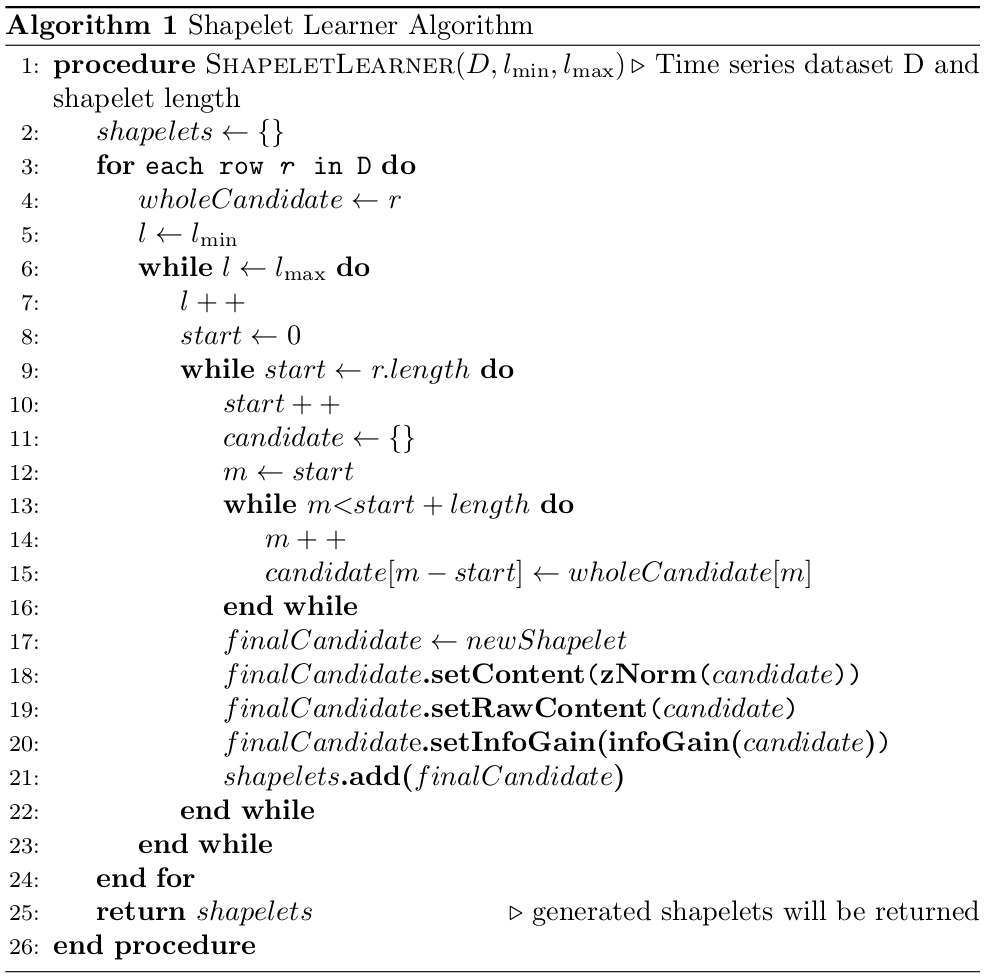
\includegraphics[width=0.5\textwidth]{algo1.png}
\end{figure}
\begin{figure}
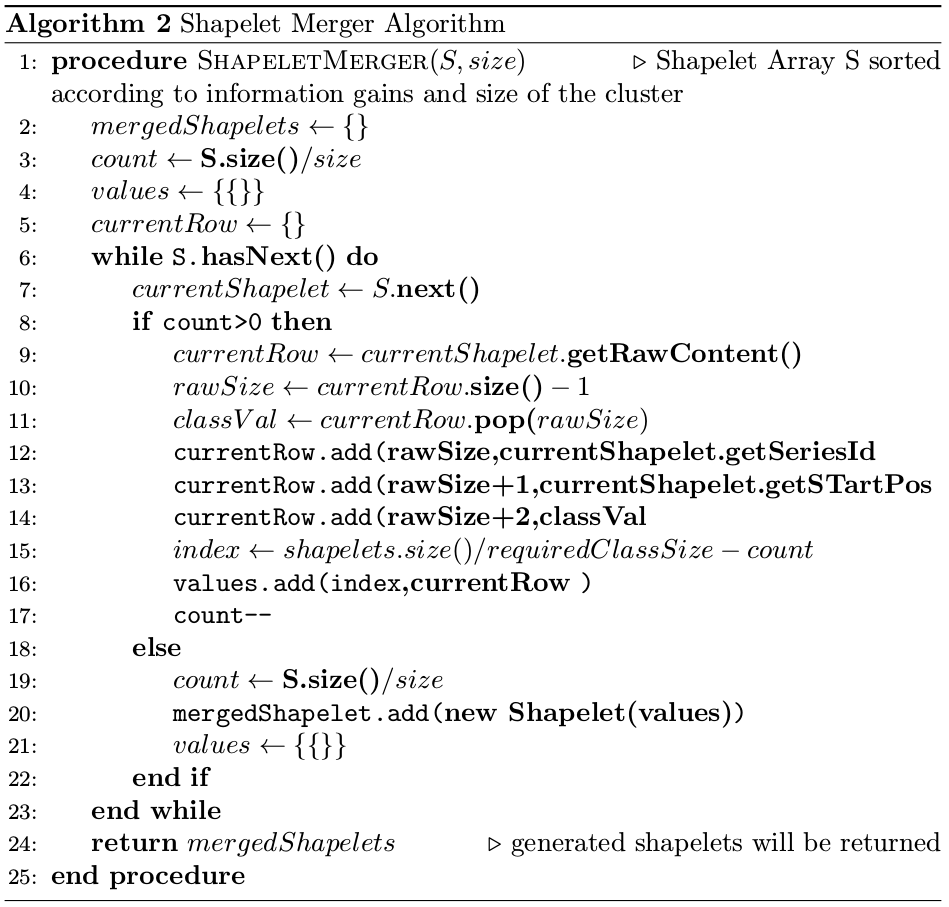
\includegraphics[width=0.5\textwidth]{algo2.png}
\end{figure}

Each shapelet of the $mergedShapelets$ array will have three additional variables. They are as follows
\begin{itemize}
\item Class value
\item Starting position
\item Series ID
\end{itemize}

\textit{Important Shapelet Finder} algorithm (Algorithm 3) takes in three parameters, namely Merged Shapelets, Class Values (Event), and Classified dataset. Line 2 and 3 initialize two lists named \textit{shapletArr} and \textit{classValueProb} which would respectively contain important shapelets and probabilities for class values within the total dataset. Then for each class value, a \textit{set} data structure is created named \textit{shapeletBucket}. \textit{findProb()} function calculates the probability of the relevant class values within the dataset. In the next step, each merged shapelet is included into a relevant \textit{shapeletBucket} by \textit{maxProbClassVal()} function. The function \textit{maxProbClassVal()} produces most probable class values for each group of shapelets. Next, the algorithm 3 finds the absolute differences between the probabilities of actual events of the dataset and groups of shapelets where the absolute difference is calculated using the \textit{getMinDifShape()} function. Since the chosen group of shapelet per each event comprises the minimum difference with respect to the actual event distribution in the dataset, it enables us to choose the most representative groups of shapelets per each event. Finally, the extracted group of shapelets are added to the \textit{shapeletArr}. Here the class value represents an event of the obtained dataset.

Regardless of the CEP query language, two blocks are needed to generate a meaningful CEP query for an event. First, the timeFrame (or window) of the rule need to be identified from the extracted shapelets. This will be defined using the \textit{within} construct. Second, the conditions that need to be met on the captured sequence of events in order for the rule to be fired, where the correspond block is defined using the where construct. 
\vspace{0.1cm}
\begin{equation}
\textbf{within}[window] \textbf{where}[conditions]
\label{eq:withinWhere}
\end{equation}
 The \textit{conditions} are extracted using the selected attributes and their respective value regions of the important shapelets. If user wants to get a CEP rule to identify multiple events, in addition to above two blocks, \textbf{filter} block should be there. Filter block will be written between two curly brackets \textbf{\{\}}
\begin{equation}
\textbf{within}[window] \{relevent events\} \textbf{where}[conditions]
\label{eq:releventEvents}
\end{equation}

\begin{figure}
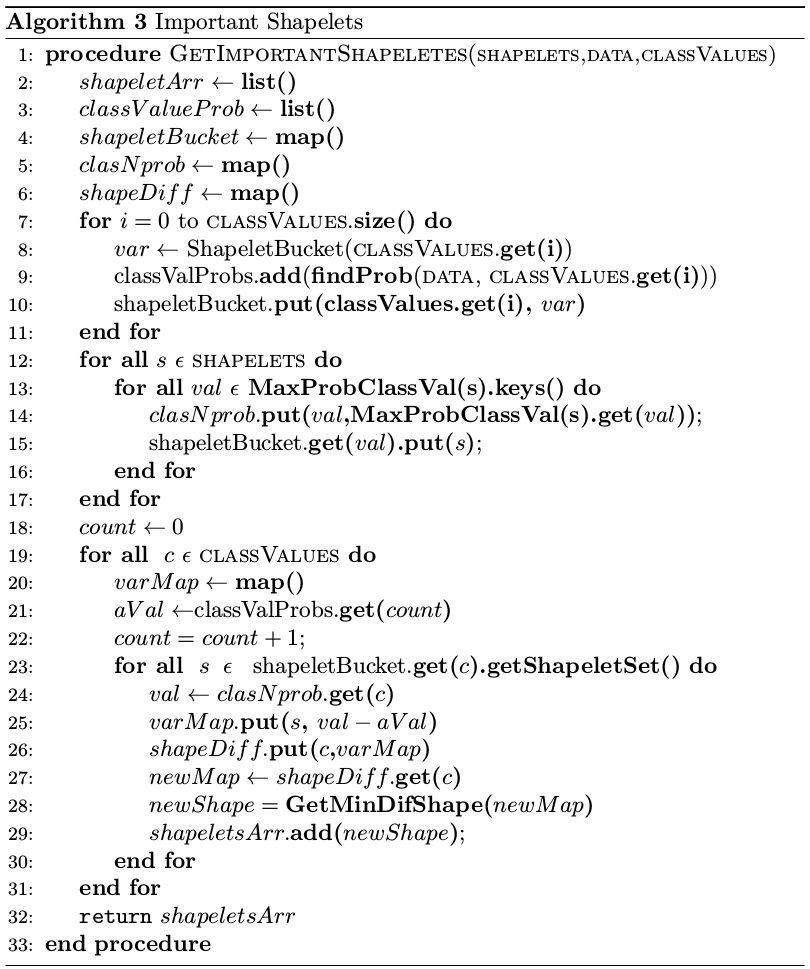
\includegraphics[width=0.5\textwidth]{algo3.png}
\end{figure}

\section{Performance Analysis}
We present detailed performance evaluation of automating query generation for CEP using shapelets and parallel coordination. We use two multivariate time series datasets from UCI machine learning repository \cite{IEEEexample:Ocupancy,IEEEexample:EEG} for evaluation purposes to prove that our technique can automate CEP query generation for different types of domains.

\subsection{Occupancy Dataset} 
“Occupancy Detection” dataset \cite{IEEEexample:Ocupancy} is a multivariate time-series dataset of which measure the occupancy factor of an office room with respect to light, temperature, humidity and CO2 measurements. It consists of 8,143 instances out of which 6,414 (78\%) instances are labeled as not occupied (occupancy = 0) while the rest (1,729 or 21\%) is labeled as occupied (occupancy = 1). Our objective was to auto generate queries to detect the occupied event as well as not occupied event along with a timely representation.

This dataset results in 9,344 shapelets, and then the most appropriate shapelets are filtered out and used for the query generation process. Fig.~\ref{fig:occupancyEvent1} and Fig.~\ref{fig:occupancyEvent2} illustrates the most appropriate shapelets to detect occupied and non-occupied events. Most appropriate shapelets from Fig.~\ref{fig:occupancyEvent1} are within attribute 1 and attribute 3. The generated query will consist of the relevant attributes and it ranges with the optimal event detection time frame. Table \rom{1} summarizes the accuracy of detected events based on the auto generated queries.  


\begin{figure}
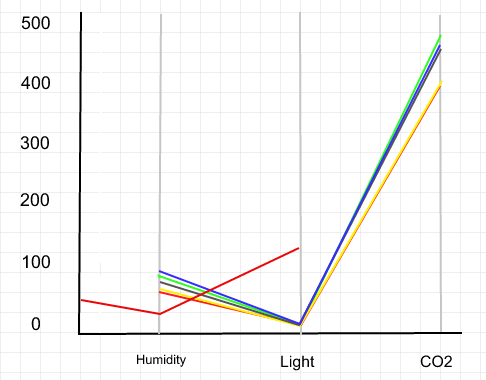
\includegraphics[width=0.5\textwidth]{Occupancy_event1.png}
\caption{"Non-Occupancy" event detected shapelets.}
\label{fig:occupancyEvent1}
\end{figure}

\begin{figure}
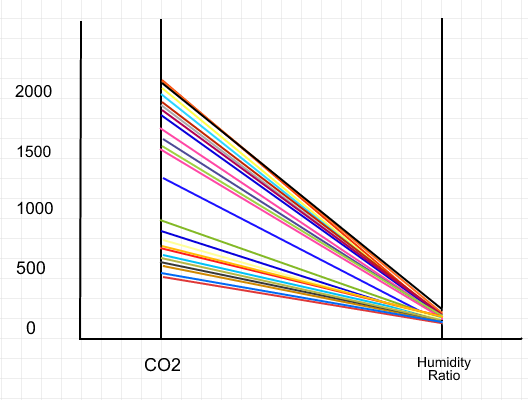
\includegraphics[width=0.5\textwidth]{Occupancy_event2.png}
\caption{"Occupied" event detected shapelets.}
\label{fig:occupancyEvent2}
\end{figure}


We have considered the time windows as follows:
\begin{itemize}
\item Non Occupied Events (\textbf{occupancy=0}) considered time window (\textbf{time window 1}) : 2015-02-08 : 17:32:00 - 22:23:00
\item Occupied Events (\textbf{occupancy=1}) considered time window (\textbf{time window 2}) : 2015-02-09 : 14:49:00 - 18:40:00
\end{itemize}

\begin{table}
\begin{center}
\caption{Occupancy dataset event detection results.}
\begin{tabular}{ | m{6cm} | m{2.3cm}| } 
 \hline 
\textbf{Description} & \multicolumn{1}{|r|}{\textbf{Value}}\\
\hline
No of non-occupied events within time windows 1 & \multicolumn{1}{|r|}{291}\\
\hline
No of non-occupied events detected using generated CEP query & \multicolumn{1}{|r|}{286}\\
\hline
Recall of non-occupied event detection & \multicolumn{1}{|r|}{98.28\%}\\
\hline
Precision of non-occupied event detection & \multicolumn{1}{|r|}{100.00\%}\\
\hline
False positives for non-occupied event detection & \multicolumn{1}{|r|}{0}\\
\hline
False negatives for non-occupied event detection & \multicolumn{1}{|r|}{5 (1.72\%)}\\
\hline
No of occupied within time window 2 & \multicolumn{1}{|r|}{196} \\
\hline
No of occupied events detected using generated CEP query & \multicolumn{1}{|r|}{196}\\ 
 \hline
Recall of occupied event detection & \multicolumn{1}{|r|}{100.00\%}\\
\hline
Precision of occupied event detection & \multicolumn{1}{|r|}{84.48\%}\\
\hline
False positives for occupied event detection & \multicolumn{1}{|r|}{36 (18.37\%)}\\
\hline
False negatives for non-occupied event detection & \multicolumn{1}{|r|}{0}\\
\hline

\end{tabular}
\end{center}
\end{table}

\subsection{EEG Eye state dataset}
All data is from one continuous EEG measurement with the Emotiv EEG Neuroheadset \cite{IEEEexample:EEG}. The duration of the measurement was 117 seconds. The eye state was detected via a camera during the EEG measurement and added later manually to the file after analysing the video frames. '1' indicates the eye-closed and '0' the eye-open state. All values are in chronological order with the first measured value at the top of the data. The two events which is in the occupancy dataset are detected using the identified most appropriate shapelets. Fig.~\ref{fig:EEGEvent1} and Fig.~\ref{fig:EEGevent2} corresponds to the most appropriate shapelets to detect event 1 and event 2. The generated query will consist of the relevant attributes and it ranges with the optimal event detection time frame. Table \rom{2} summarizes the accuracy of detected events based on the auto generated queries.

\begin{figure}[h!]
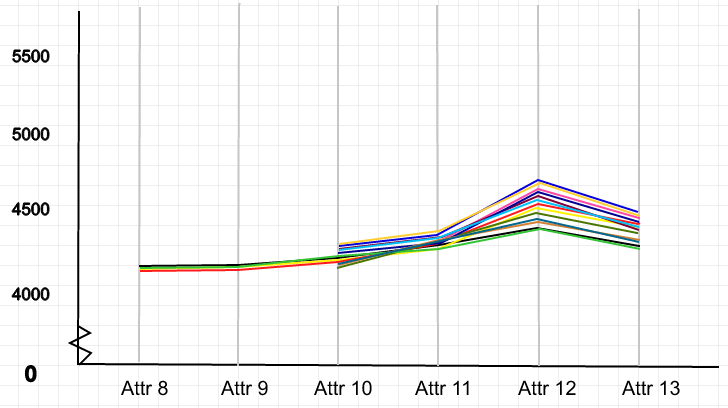
\includegraphics[width=0.5\textwidth]{EEG_event1.png}
\caption{EEG eye state open event detected shapelets.}
\label{fig:EEGEvent1}
\end{figure}

\begin{figure}[h!]
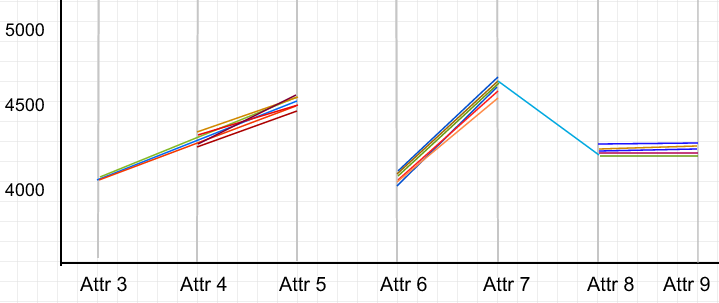
\includegraphics[width=0.5\textwidth]{EEG_event2.png}
\caption{EEG eye state close event detected shapelets.}
\label{fig:EEGevent2}
\end{figure}

Table \rom{2} displays a summarized representation of the obtained accuracy values of the generated queries for eye open and close events of the EEG Eye state dataset.

We have considered the time windows as follows:
\begin{itemize}
\item Event - \textbf{Eye State Open} considered time window (time window 1) : 128349s to 204516s
\item Event - \textbf{Eye State Close} considered time window (time window 2):
14976s to 128232s
\end{itemize}

\begin{table}
\caption{EEG Eye State dataset event detection results.}
\begin{center}
\begin{tabular}{ | m{6cm} | m{2.3cm}| } 
 \hline 
\textbf{Description} & \multicolumn{1}{|r|}{\textbf{Value}}\\
\hline
No of eye state open events within time window 1 & \multicolumn{1}{|r|}{652}\\
\hline
No of eye state open events detected using generated CEP query & \multicolumn{1}{|r|}{635}\\
\hline
Recall of eye state open event detection & \multicolumn{1}{|r|}{97.39\%}\\
\hline
Precision of eye state open event detection & \multicolumn{1}{|r|}{100.00\%}\\
\hline
False positives for eye state open event detection & \multicolumn{1}{|r|}{0}\\
\hline
False negatives for eye state open event detection & \multicolumn{1}{|r|}{17 (2.67\%)}\\
\hline
No of eye state close events within time window 2 & \multicolumn{1}{|r|}{69}\\
\hline
No of eye state close events detected using CEP query generated & \multicolumn{1}{|r|}{68}\\
\hline
Recall of eye state close event detection & \multicolumn{1}{|r|}{98.55\%}\\
\hline
Precision of eye state close event detection & \multicolumn{1}{|r|}{100.00\%}\\
\hline
False positives for eye state close event detection & \multicolumn{1}{|r|}{0}\\
\hline
False negatives for eye state close event detection & \multicolumn{1}{|r|}{1 (1.45\%)}\\
\hline

\end{tabular}
\end{center}
\end{table}

\section{Summary and Future Work}

Proposed solution identifies shapelets in the whole dataset and store relevant attributes for each shapletes. Information gain, Starting position and Shapelets contents are important attributes for further processes. First phase of the solution does this shapelets learning process using shapelet learning algorithm. Second phase is related with the classified values of the dataset where it finds a relationship with shapelets and the classified dataset. It happens by comparing information gains and probabilities of occurrences of shapletes. In future we plan to extend the proposed technique work with unlabeled datasets, as well as optimize the information gain calculation procedure, shapelet learner, and shapelet extraction techniques.

\nocite{*}
\bibliographystyle{IEEEtran}
\bibliography{IEEEabrv,IEEEexample}

\end{document}
